\section{Gradient-based learning}

\begin{frame}\frametitle{\secname}
	Training error $E^T$ for the training set $\left\{\vec x^{(\alpha)}, y^{(\alpha)}_{T}\right\}$: 
    \begin{equation}
        \ETw = \frac{1}{p} \sum\limits_{\alpha = 1}^p 
					e\tyxwalpha
    \end{equation}
    
    \mode<article>{
    The objective is to minimize the training error w.r.t. the model parameters $\vec w$. That is
    }
    
    \begin{equation}
        \ETw \eqexcl \min_{\vec w} \quad \Rightarrow \quad \vec w^{*} = \argmin_{\vec w} \ETw
    \end{equation}

    \begin{figure}[h]
        \centering
        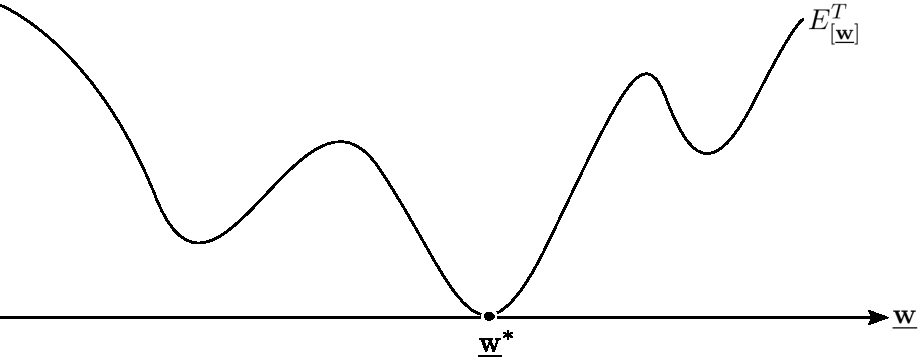
\includegraphics[height=3.25cm]{img/section1_fig19_no_steps}
        \caption{Training error with minimum at $\vec w^{*}$}
        \label{fig:training_error} 
    \end{figure}
    
    \pause 
    
    \question{What is the strategy for finding $\vec w^{*}$ analytically?}
    

    
    
\end{frame}

\begin{frame}\frametitle{Finding the minumum of $\ETw$ analytically}

    Example with a simple connectionist neuron model
    with parameters
    $$\vec w = (w_{0}, w_{1}, \ldots, w_{N})^{\top}$$\\


    - The strategy for finding the minimum of a function $E_{[\vec{w}]}^T$ analytically is as follows:
    \begin{enumerate}
    \item Compute the gradient w.r.t. $\vec w$ by taking the first partial derivatives w.r.t to each component in the vector $\vec w$
    \begin{equation}
        \frac{\partial \ETw}{\partial \vec w} = \left(\,
        \frac{\partial \ETw}{\partial w_{0}}, \,
        \frac{\partial \ETw}{\partial w_{1}}, \,\ldots\,,\, 
        \frac{\partial \ETw}{\partial w_{N}}\,
        \right)^{\top}
        \label{eq:gradient_partial}
    \end{equation}
    The gradient $\frac{\partial \ETw}{\partial \vec w}$ has the same dimensionality as $\vec w$.
    
    \item Set the gradient to zero: $\frac{\partial \ETw}{\partial \vec w} \eqexcl \vec 0$
    \item Solve for $\vec w$ to find extrema.
    \item Select solution corresponding to global minimum.
    
    \end{enumerate}
    \mode<presentation>{
    Caveat: Not always applicable. Closed-form solution infeasible for complex models such as MLPs.
    Instead: Iterative learning algorithm gradient descent.
    }
\end{frame}


\begin{frame}\frametitle{Finding the minumum of $\ETw$ iteratively}

\mode<article>{

Learning from gradient descent is an alternate approach for finding the minimum of a function, when the closed-form solution is not available.

}
    \begin{figure}[h]
        \centering
        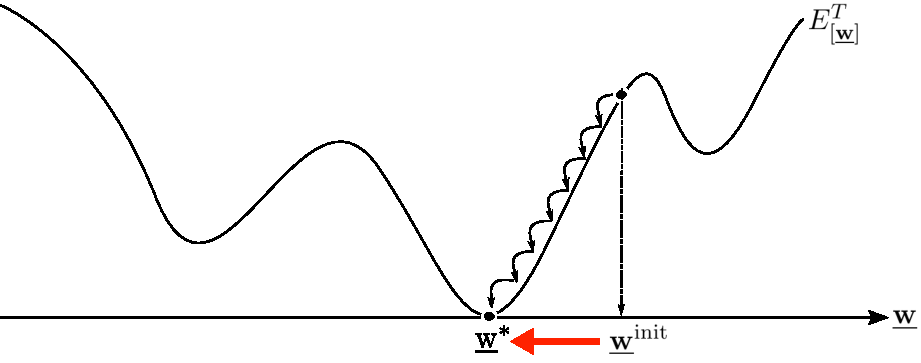
\includegraphics[height=3.25cm]{img/section1_fig19}
        \caption{Minimzing the training error iteratively via gradient descent}
        \label{fig:minimize_via_gradient_descent} 
    \end{figure}
    
    \only<1>{
    For our connectionist neuron example:
    \begin{equation}
    		w_{i}(t+1) \quad=\quad w_{i}(t) 
				\;\;{\color{red}-}\;\;
				\underbrace{{\eta}}_{ 
						\substack{\text{learning} \\ \text{step} } }
                        \cdot
				\underbrace{\frac{\partial \ETw}{
					\partial \mathrm{w}_{i}}}_{
						\substack{
							\text{\textcolor{red}{``gradient''}} 
			} }
            \label{eq:gradient_descent_neuron}
    \end{equation}
    
    $\vec w^{\mathrm{init}}$ is bascially a random guess of where the solution might be and going against the gradient will potentially move us closer to the minimum. 
    }
	\only<2,3>{
    For an MLP:
    \begin{equation}
		w_{ij}^{v'v}(t+1) \quad=\quad w_{ij}^{v'v}(t) 
				\;\;{\color{red}-}\;\;
				\underbrace{\eta}_{ 
						\substack{\text{learning} \\ \text{step} } }
                        \cdot
				\underbrace{\frac{\partial \ETw}{
					\partial \mathrm{w}_{ij}^{v'v}}}_{
						\substack{
							\text{\textcolor{red}{gradient vector}} 
			} }
            \label{eq:gradient_descent_mlp}
    \end{equation}
    }
    
    \mode<article>{
    
    The learning step (learning rate) $\eta$ modulates the magnitude of our update. $\eta$ can be treated as a constant but we will also see how the value of $\eta$ can change over time, i.e. $\eta(t)$.
    }
    \only<3>{
    \question{Why do we \underline{subtract} the gradient from the current value of $w_{ij}^{v'v}(t)$?}
    }
    
    \mode<article>{
    
    The gradient describes the slope. Adding it will move us upwards and potentially maximize our function. Gradient-based learning with the intention of maximizing some function is referred to as hill climbing or gradient \emph{ascent}.
    }
    
    \only<4>{
    \question{So what's the downside of using gradient descent?}\\
    }
\end{frame}

\mode<article>{

    - The solution we find heavily depends on the initial position we started from. Indeed, gradient descent will reduce our cost each step but it does not guarantee that it will find the global minimum and will also stop at a local minimum. The slope in both cases is equal to zero.
    }

\begin{frame}
    \mode<presentation>{
    
    \textbf{So what's the downside of using gradient descent?}\\
    
    }
    
    \begin{figure}[h]
        \centering
        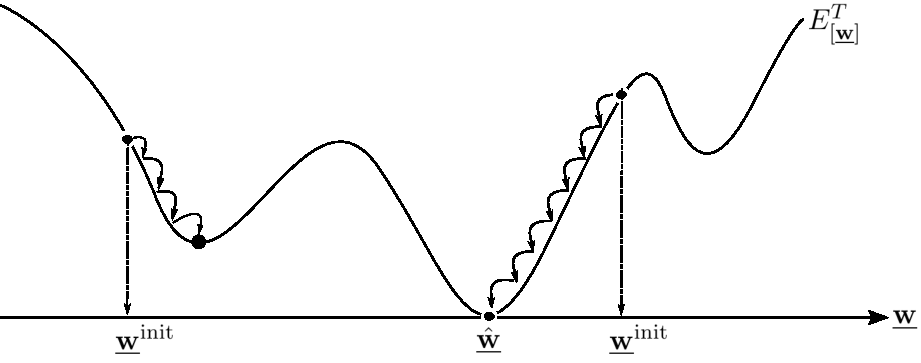
\includegraphics[height=3.25cm]{img/section1_fig19_local}
        \caption{Gradient descent finds local minima.}
        \label{fig:minimize_via_gradient_descent_local} 
    \end{figure}
    
\end{frame}
